        \clearpage
        \begin{figure*}[ht]
            \pdfbookmark[2]{ID 03}{figure_id_03}
        	\centering
            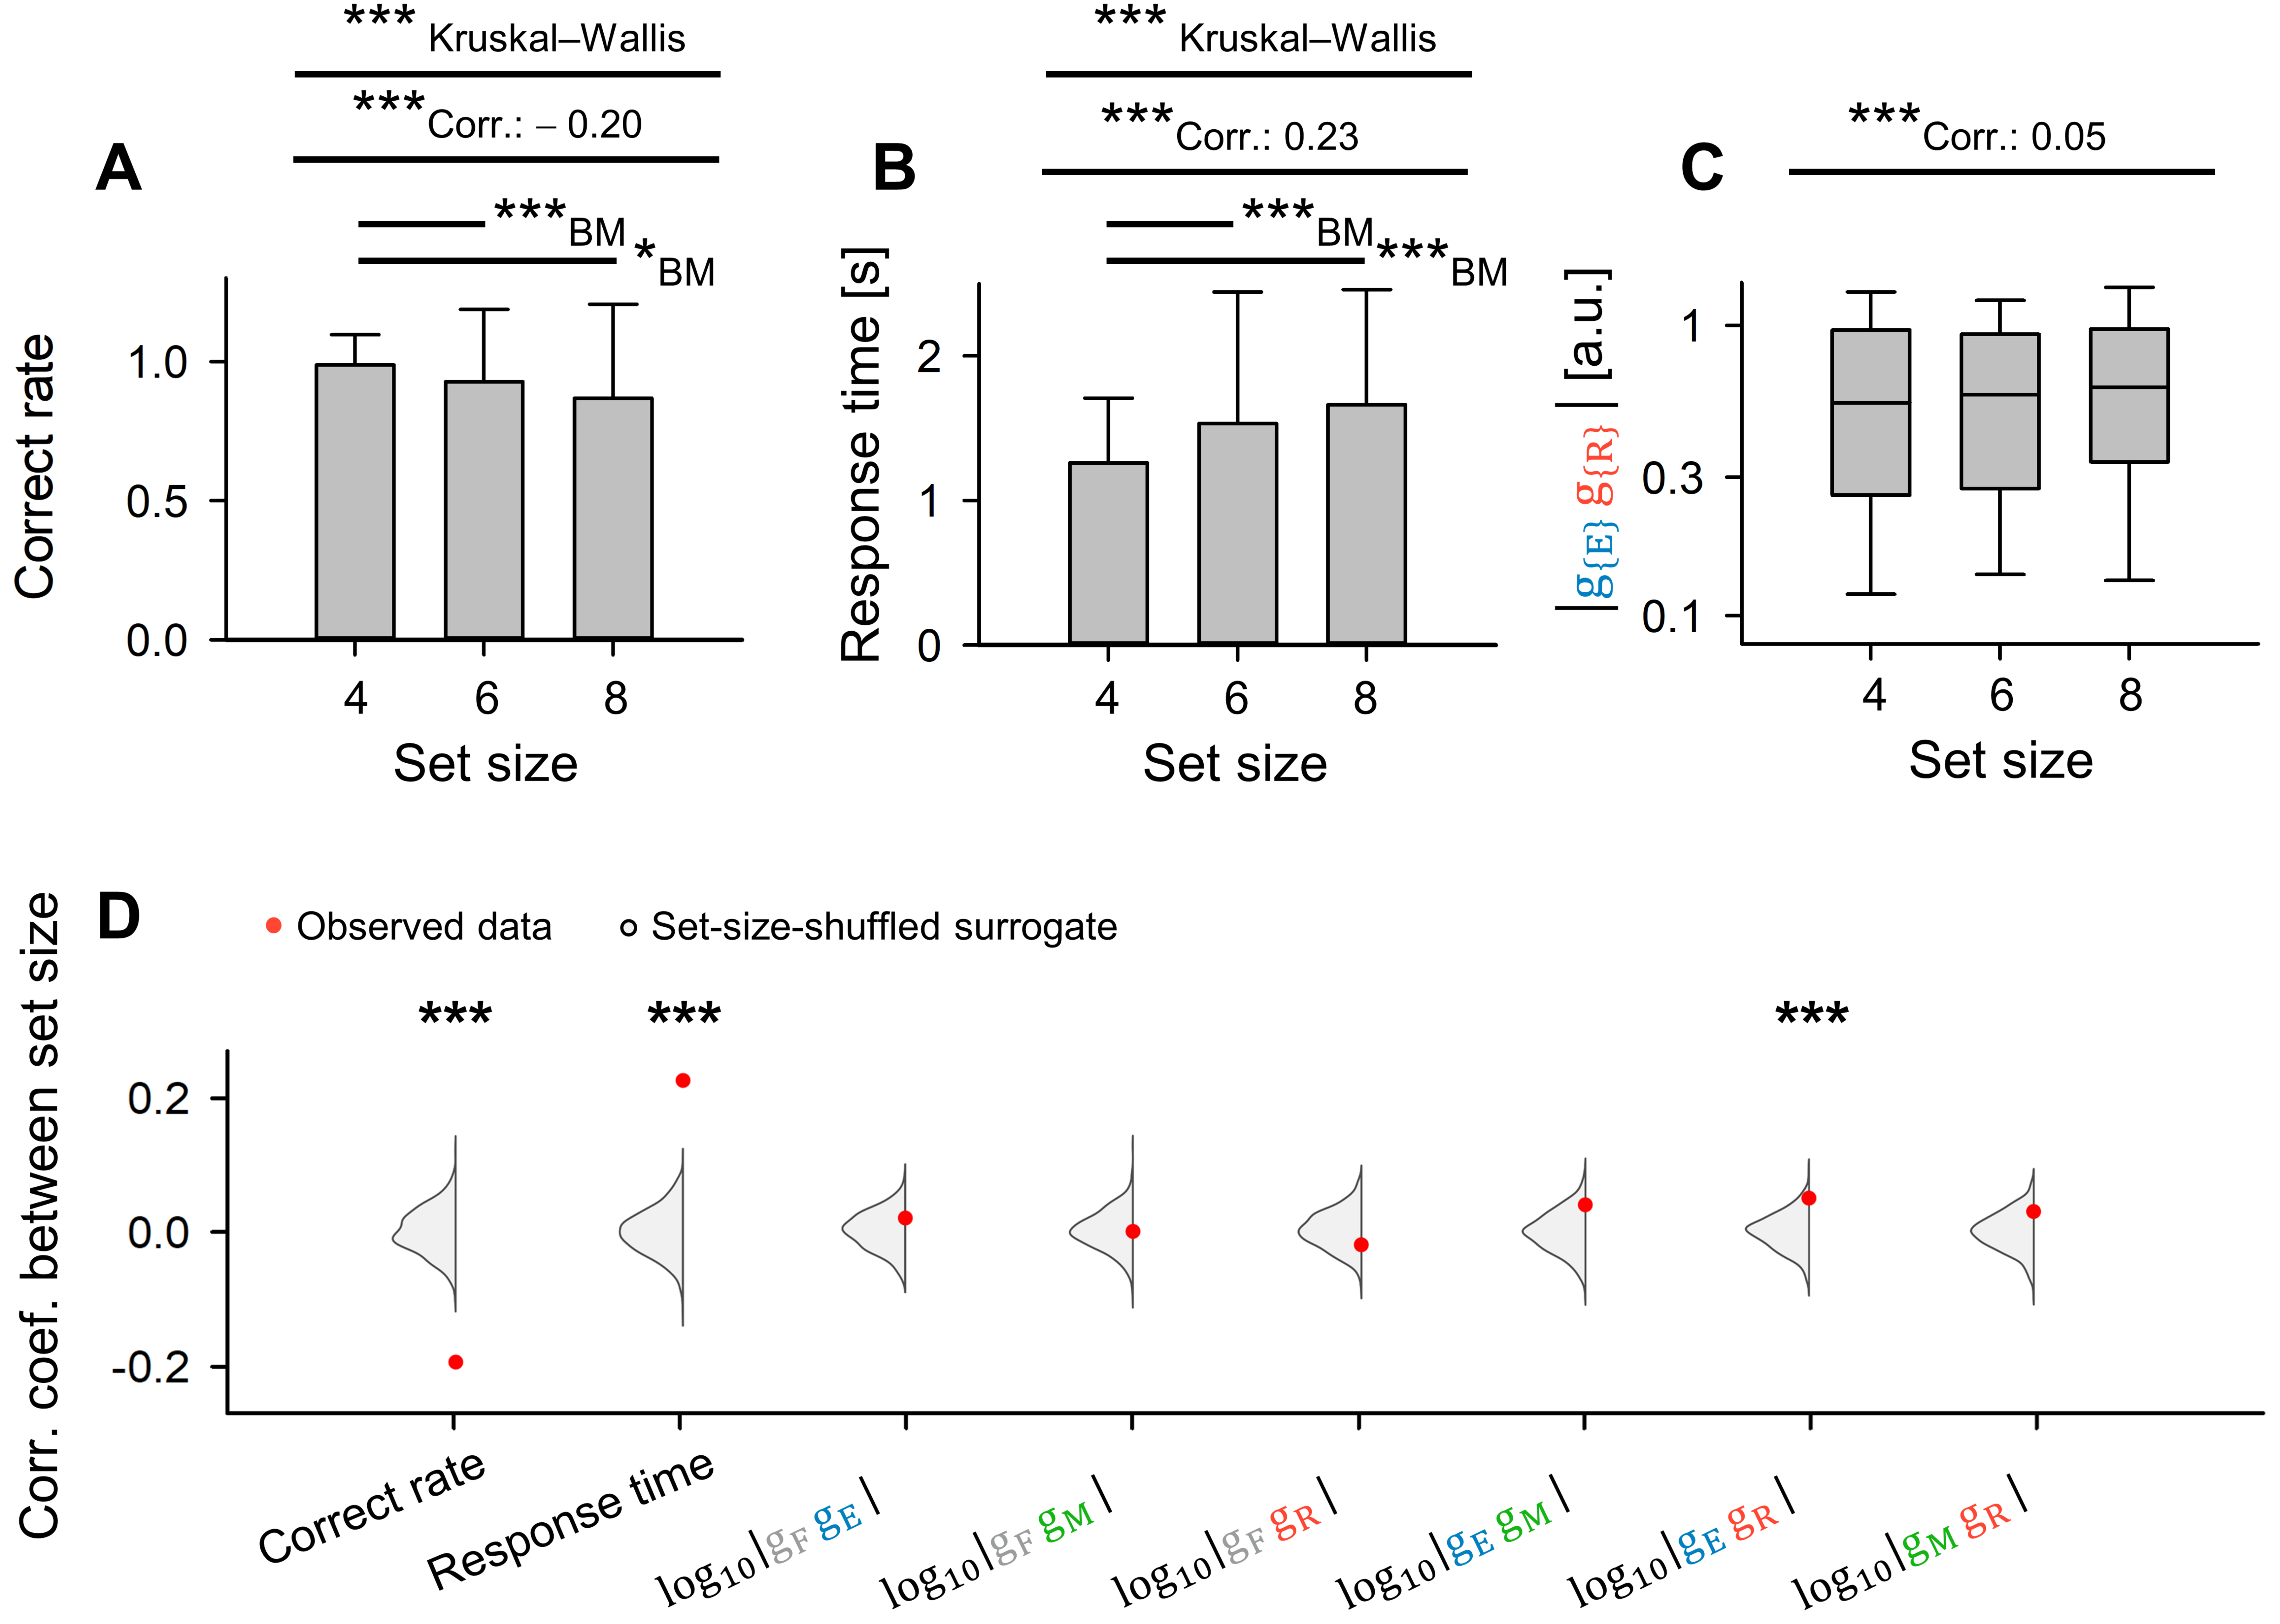
\includegraphics[width=1\textwidth]{./src/figures/.png/Figure_ID_03.png}
        	\caption{\textbf{
Memory-load dependency in trajectory distance between encoding and retrieval states in the hippocampus 
}
\smallskip
\\
\textbf{\textit{A.}} Set size (number of letters to encode) and correct rate in the WM task (coefficient = $-0.20$, ***\textit{p} $<$ 0.001). \textbf{\textit{B.}} Set size and response time (coefficient = 0.23, ***\textit{p} $<$ 0.001).  \textbf{\textit{C.}} Set size and the inter-phase distances between encoding and retrieval phases ($\lVert \mathrm{g_{E}g_{R}} \rVert$) (correlation coefficient = 0.05). \textbf{\textit{D.}} \textit{Red} dots show experimentally observed correlations between set size and the following parameters: correct rate, response time, $\log_{10}{\lVert \mathrm{g_{F}g_{E}} \rVert}$, $\log_{10}{\lVert \mathrm{g_{F}g_{M}} \rVert}$, $\log_{10}{\lVert \mathrm{g_{F}g_{R}} \rVert}$, $\log_{10}{\lVert \mathrm{g_{E}g_{M}} \rVert}$, $\log_{10}{\lVert \mathrm{g_{E}g_{R}} \rVert}$, and $\log_{10}{\lVert \mathrm{g_{M}g_{R}} \rVert}$. The \textit{gray} kernel density plot shows corresponding set-size-shuffled surrogate (\textit{n} = 1,000) (***\textit{p}s $<$ 0.001).
}
% width=1\textwidth
        	\label{fig:03}
        \end{figure*}
